% Options for packages loaded elsewhere
\PassOptionsToPackage{unicode}{hyperref}
\PassOptionsToPackage{hyphens}{url}
%
\documentclass[
]{article}
\usepackage{amsmath,amssymb}
\usepackage{iftex}
\ifPDFTeX
  \usepackage[T1]{fontenc}
  \usepackage[utf8]{inputenc}
  \usepackage{textcomp} % provide euro and other symbols
\else % if luatex or xetex
  \usepackage{unicode-math} % this also loads fontspec
  \defaultfontfeatures{Scale=MatchLowercase}
  \defaultfontfeatures[\rmfamily]{Ligatures=TeX,Scale=1}
\fi
\usepackage{lmodern}
\ifPDFTeX\else
  % xetex/luatex font selection
\fi
% Use upquote if available, for straight quotes in verbatim environments
\IfFileExists{upquote.sty}{\usepackage{upquote}}{}
\IfFileExists{microtype.sty}{% use microtype if available
  \usepackage[]{microtype}
  \UseMicrotypeSet[protrusion]{basicmath} % disable protrusion for tt fonts
}{}
\makeatletter
\@ifundefined{KOMAClassName}{% if non-KOMA class
  \IfFileExists{parskip.sty}{%
    \usepackage{parskip}
  }{% else
    \setlength{\parindent}{0pt}
    \setlength{\parskip}{6pt plus 2pt minus 1pt}}
}{% if KOMA class
  \KOMAoptions{parskip=half}}
\makeatother
\usepackage{xcolor}
\usepackage[margin=1in]{geometry}
\usepackage{longtable,booktabs,array}
\usepackage{calc} % for calculating minipage widths
% Correct order of tables after \paragraph or \subparagraph
\usepackage{etoolbox}
\makeatletter
\patchcmd\longtable{\par}{\if@noskipsec\mbox{}\fi\par}{}{}
\makeatother
% Allow footnotes in longtable head/foot
\IfFileExists{footnotehyper.sty}{\usepackage{footnotehyper}}{\usepackage{footnote}}
\makesavenoteenv{longtable}
\usepackage{graphicx}
\makeatletter
\def\maxwidth{\ifdim\Gin@nat@width>\linewidth\linewidth\else\Gin@nat@width\fi}
\def\maxheight{\ifdim\Gin@nat@height>\textheight\textheight\else\Gin@nat@height\fi}
\makeatother
% Scale images if necessary, so that they will not overflow the page
% margins by default, and it is still possible to overwrite the defaults
% using explicit options in \includegraphics[width, height, ...]{}
\setkeys{Gin}{width=\maxwidth,height=\maxheight,keepaspectratio}
% Set default figure placement to htbp
\makeatletter
\def\fps@figure{htbp}
\makeatother
\setlength{\emergencystretch}{3em} % prevent overfull lines
\providecommand{\tightlist}{%
  \setlength{\itemsep}{0pt}\setlength{\parskip}{0pt}}
\setcounter{secnumdepth}{5}
\usepackage{booktabs}
\usepackage{longtable}
\usepackage{array}
\usepackage{multirow}
\usepackage{wrapfig}
\usepackage{float}
\usepackage{colortbl}
\usepackage{pdflscape}
\usepackage{tabu}
\usepackage{threeparttable}
\usepackage{threeparttablex}
\usepackage[normalem]{ulem}
\usepackage{makecell}
\usepackage{xcolor}
\ifLuaTeX
  \usepackage{selnolig}  % disable illegal ligatures
\fi
\IfFileExists{bookmark.sty}{\usepackage{bookmark}}{\usepackage{hyperref}}
\IfFileExists{xurl.sty}{\usepackage{xurl}}{} % add URL line breaks if available
\urlstyle{same}
\hypersetup{
  pdftitle={Course Evaluation Results},
  hidelinks,
  pdfcreator={LaTeX via pandoc}}

\title{Course Evaluation Results}
\author{}
\date{\vspace{-2.5em}}

\begin{document}
\maketitle

{
\setcounter{tocdepth}{2}
\tableofcontents
}
\begin{longtable}[]{@{}
  >{\raggedright\arraybackslash}p{(\columnwidth - 2\tabcolsep) * \real{0.5488}}
  >{\raggedright\arraybackslash}p{(\columnwidth - 2\tabcolsep) * \real{0.4512}}@{}}
\toprule\noalign{}
\begin{minipage}[b]{\linewidth}\raggedright
Key
\end{minipage} & \begin{minipage}[b]{\linewidth}\raggedright
Value
\end{minipage} \\
\midrule\noalign{}
\endhead
\bottomrule\noalign{}
\endlastfoot
\textbf{Course} & Business Intelligence II \\
\textbf{Course Code} & BBT4206 \\
\textbf{Class} & BBIT 4.2 \\
\textbf{Semester Duration} & 21\textsuperscript{st} August 2023 to
28\textsuperscript{th} November 2023 \\
\textbf{Date of Evaluation} &
\begin{minipage}[t]{\linewidth}\raggedright
25\textsuperscript{th} September 2023 to 29\textsuperscript{th}
September 2023\\
(Week 6/14)\strut
\end{minipage} \\
\textbf{Total number of students who submitted the course evaluation} &
94 \\
\textbf{Total number of students registered in the AMS at the time of
the course evaluation} & 115 \\
\textbf{Response rate} & 81.73\% \\
\textbf{e-Learning URL} &
\url{https://elearning.strathmore.edu/course/view.php?id=6599} \\
\textbf{Data collection tool URL (for access to the raw data)} &
\url{https://elearning.strathmore.edu/mod/questionnaire/view.php?id=221958} \\
\textbf{Lecturer} & Dr Allan Omondi \\
\end{longtable}

\begin{center}\rule{0.5\linewidth}{0.5pt}\end{center}

\section{Overall Course Evaluation
Score}\label{overall-course-evaluation-score}

Overall Course Evaluation Score

Mean Score

Percentage

4.3839

87.6789

Mean Score Percentage 1 4.383946 87.67892

\begin{center}\rule{0.5\linewidth}{0.5pt}\end{center}

\subsection{Course Evaluation Scores per
Group}\label{course-evaluation-scores-per-group}

The \textbf{``Average Course Evaluation Rating''} variable in the plot
below indicates the score \textbf{per group} with a baseline of 4/5.

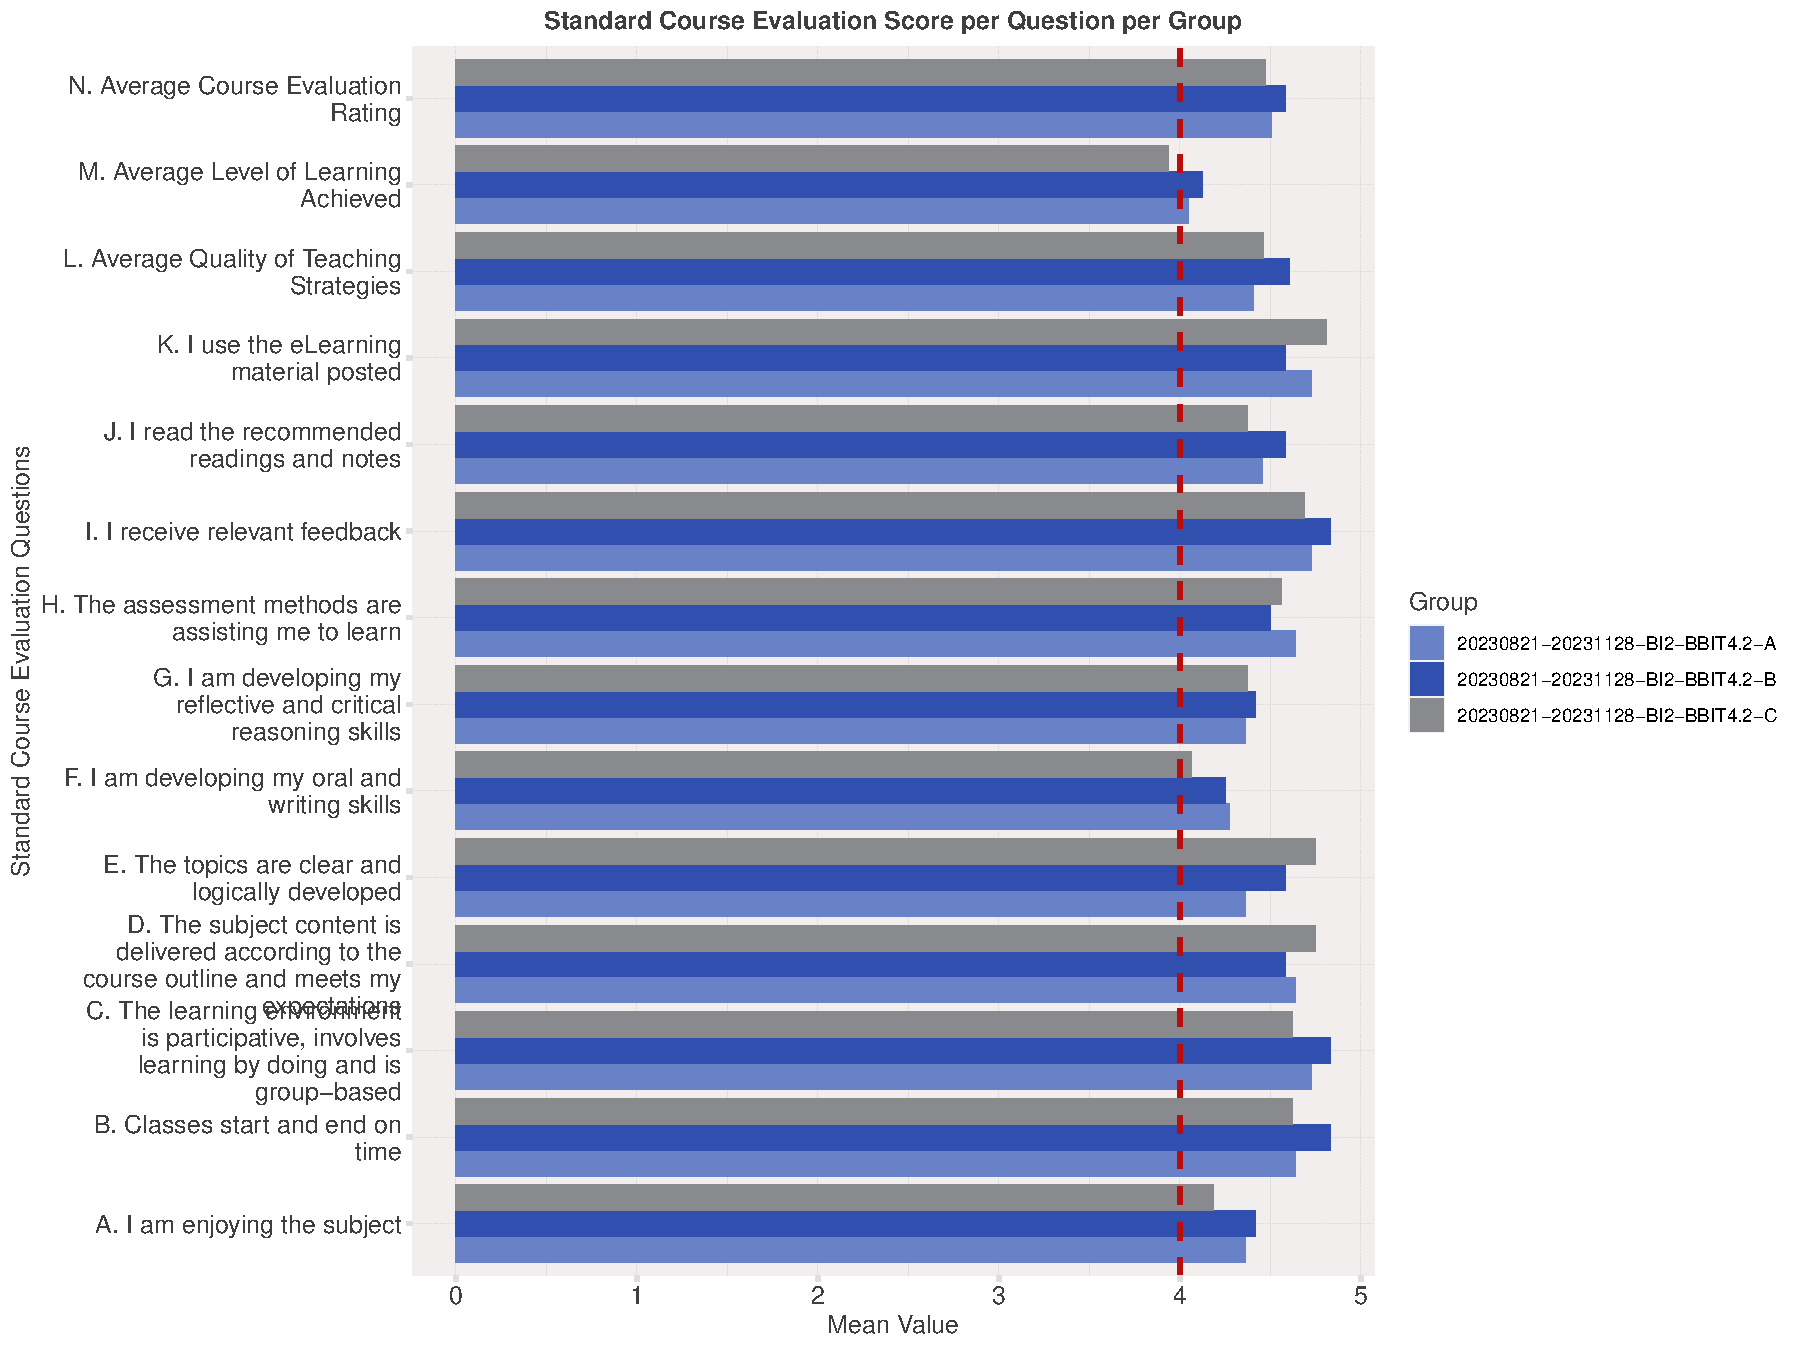
\includegraphics{AnalysisOfCourseEvaluation-Notebook_files/figure-latex/VisualizationsForCourseEvaluationResultsperClassGroup-1.pdf}

The \textbf{``Average Course Evaluation Rating''} variable in the plot
below indicates the score \textbf{per gender} with a baseline of 4/5.

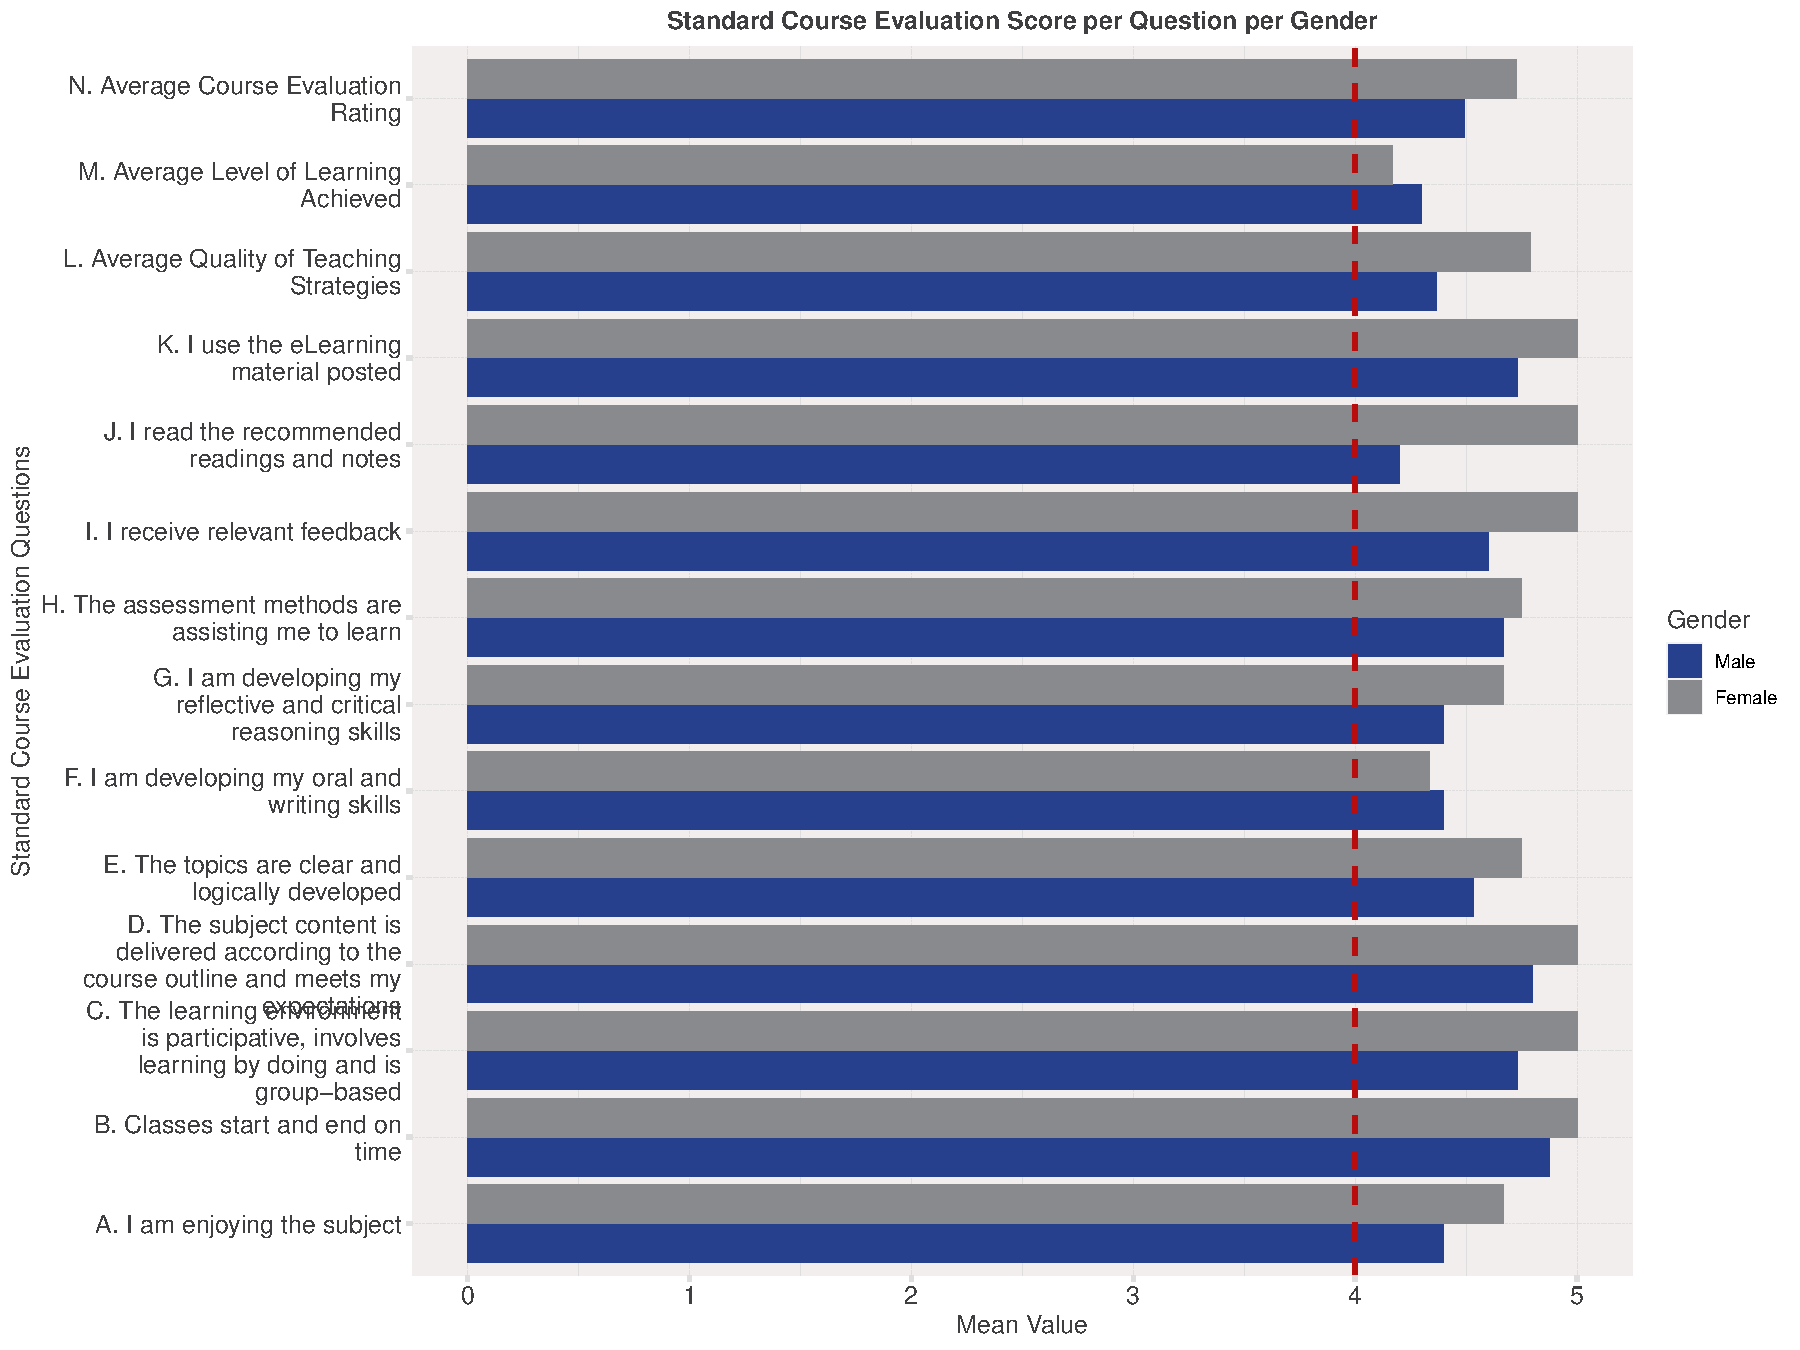
\includegraphics{AnalysisOfCourseEvaluation-Notebook_files/figure-latex/VisualizationsForCourseEvaluationResultsperGender-1.pdf}

The plot below presents a drill-down of the class group into
\textbf{regular and exempt} students:

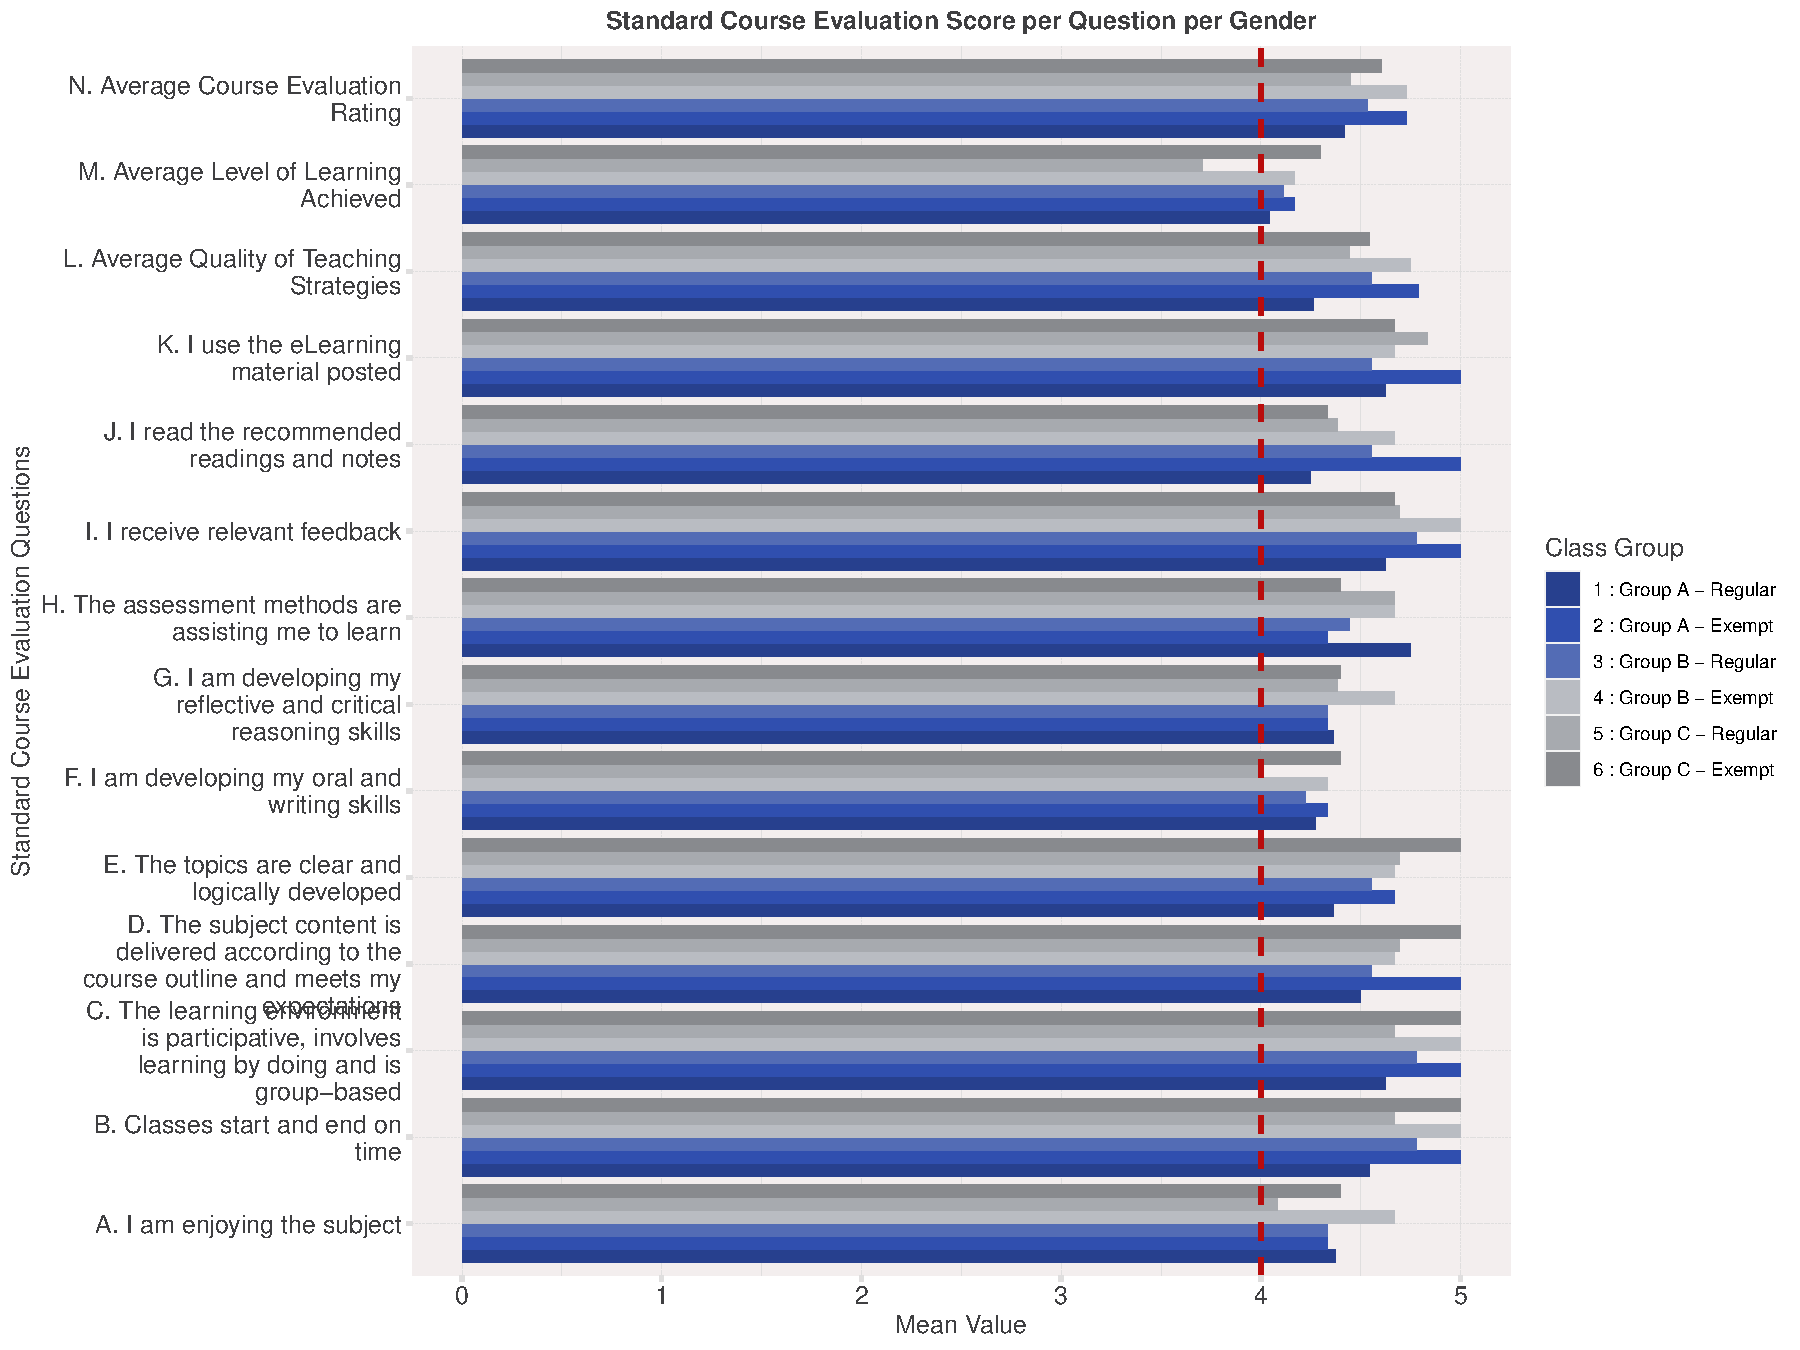
\includegraphics{AnalysisOfCourseEvaluation-Notebook_files/figure-latex/VisualizationsForCourseEvaluationResultsperGroup-1.pdf}

\section{Correlations}\label{correlations}

The following variables have been renamed to fit the correlation plots:

\begin{itemize}
\item
  `A. Enjoying Subject` = `Q02\_General Questions-\textgreater A - 1. I
  am enjoying the subject`,
\item
  `B. Classes Start-End` = `Q02\_General Questions-\textgreater A - 2.
  Classes start and end on time`,
\item
  `C. Learning Environment` = `Q02\_General Questions-\textgreater A -
  3. The learning environment is participative, involves learning by
  doing and is group-based`,
\item
  `D. Content Delivery` = `Q02\_General Questions-\textgreater A - 4.
  The subject content is delivered according to the course outline and
  meets my expectations`,
\item
  `E. Clear Topics` = `Q02\_General Questions-\textgreater A - 5. The
  topics are clear and logically developed`,
\item
  `F. Oral and Writing` = `Q02\_General Questions-\textgreater A - 6. I
  am developing my oral and writing skills`,
\item
  `G. Critical Thinking` = `Q02\_General Questions-\textgreater A - 7. I
  am developing my reflective and critical reasoning skills`,
\item
  `H. Assessment Methods` = `Q02\_General Questions-\textgreater A - 8.
  The assessment methods are assisting me to learn`,
\item
  `I. Relevant Feedback` = `Q02\_General Questions-\textgreater A - 9. I
  receive relevant feedback`,
\item
  `J. Read Recommendations` = `Q02\_General Questions-\textgreater A -
  10. I read the recommended readings and notes`,
\item
  `L. eLearning Material` = `Q02\_General Questions-\textgreater A - 11.
  I use the eLearning material posted`,
\item
  `Understood Concept 1` = `Q03\_Level of Learning
  Achieved-\textgreater B - 1. Concept 1 of 4 - Ensemble Methods for
  Predictive Analytics`,
\item
  `Understood Concept 2` = `Q03\_Level of Learning
  Achieved-\textgreater B - 2. Concept 2 of 4 - Predictive Modelling
  Using R`,
\item
  `Teaching - Labs` = `Q04\_Quality of Teaching
  Strategies-\textgreater C - 1. Labs with comments that describe each
  step to be followed`,
\item
  `Labs with Submission` = `Q04\_Quality of Teaching
  Strategies-\textgreater C - 2. Labs that require you to put in effort
  to make a submission related to the content of the lab`,
\item
  `Git in Teams` =`Q04\_Quality of Teaching Strategies-\textgreater C -
  3. Labs that require you to use Git to work in a team`,
\item
  `Solo Labs` = `Q04\_Quality of Teaching Strategies-\textgreater C - 4.
  Labs that require you to work alone`,
\item
  `Quality of Lectures` = `Q04\_Quality of Teaching
  Strategies-\textgreater C - 5. The quality of the lectures given
  (quality measured by the breadth (the full span of knowledge of a
  subject) and depth (the extent to which specific topics are focused
  upon, amplified, and explored) of learning - NOT quality measured by
  how fun/comical/lively the lectures are)`,
\item
  `Recordings of Classes` = `Q04\_Quality of Teaching
  Strategies-\textgreater C - 6. The recordings of online classes`,
\item
  `Online Classes` = `Q04\_Quality of Teaching Strategies-\textgreater C
  - 7. Online classes in general`,
\item
  `Physical Classes` = `Q04\_Quality of Teaching
  Strategies-\textgreater C - 8. Face-to-Face classes in general`
\end{itemize}

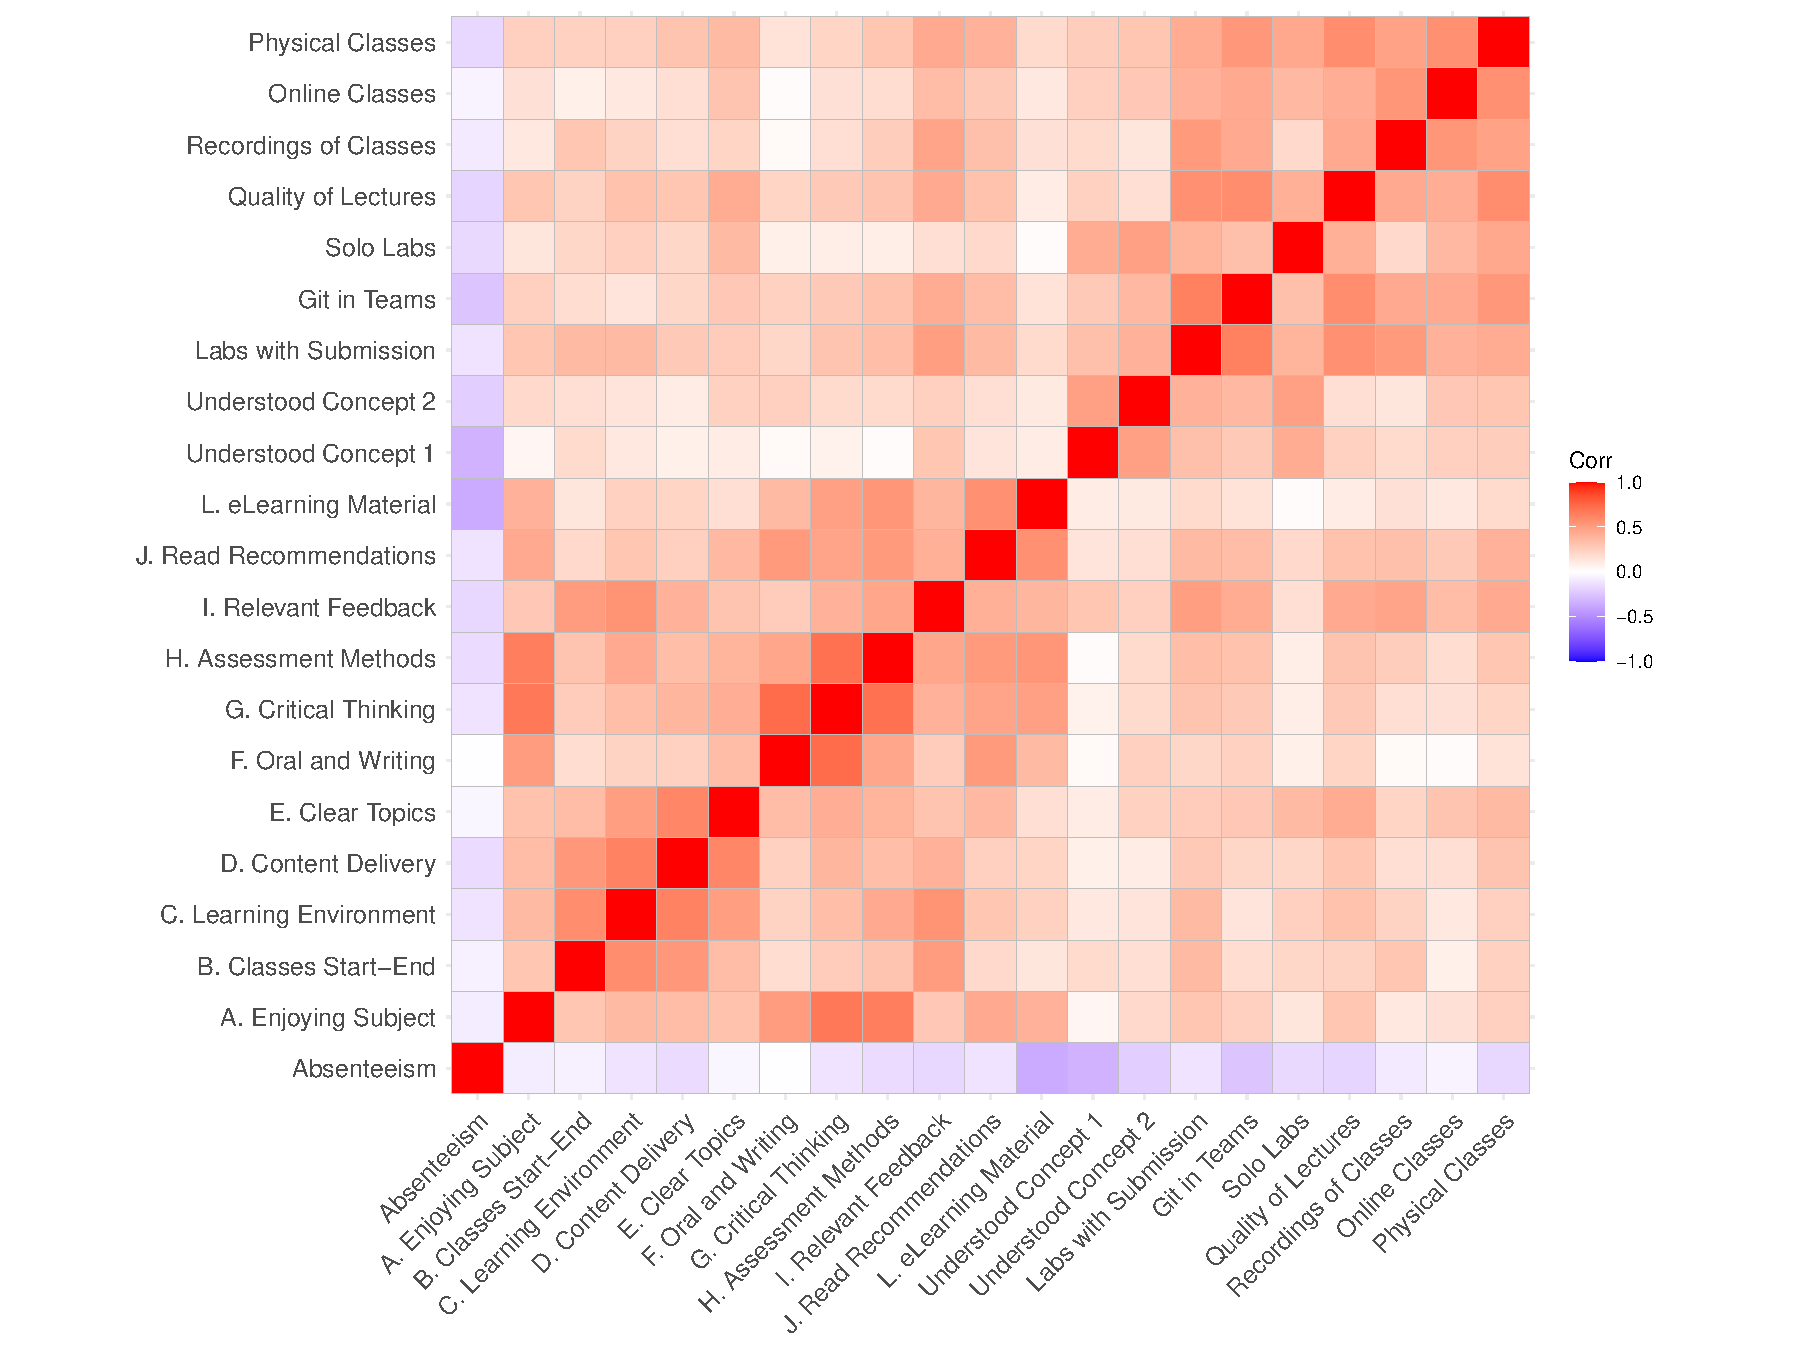
\includegraphics{AnalysisOfCourseEvaluation-Notebook_files/figure-latex/CorrelationMatrixWithoutFigures-1.pdf}

The specifc correlation values are presented below:

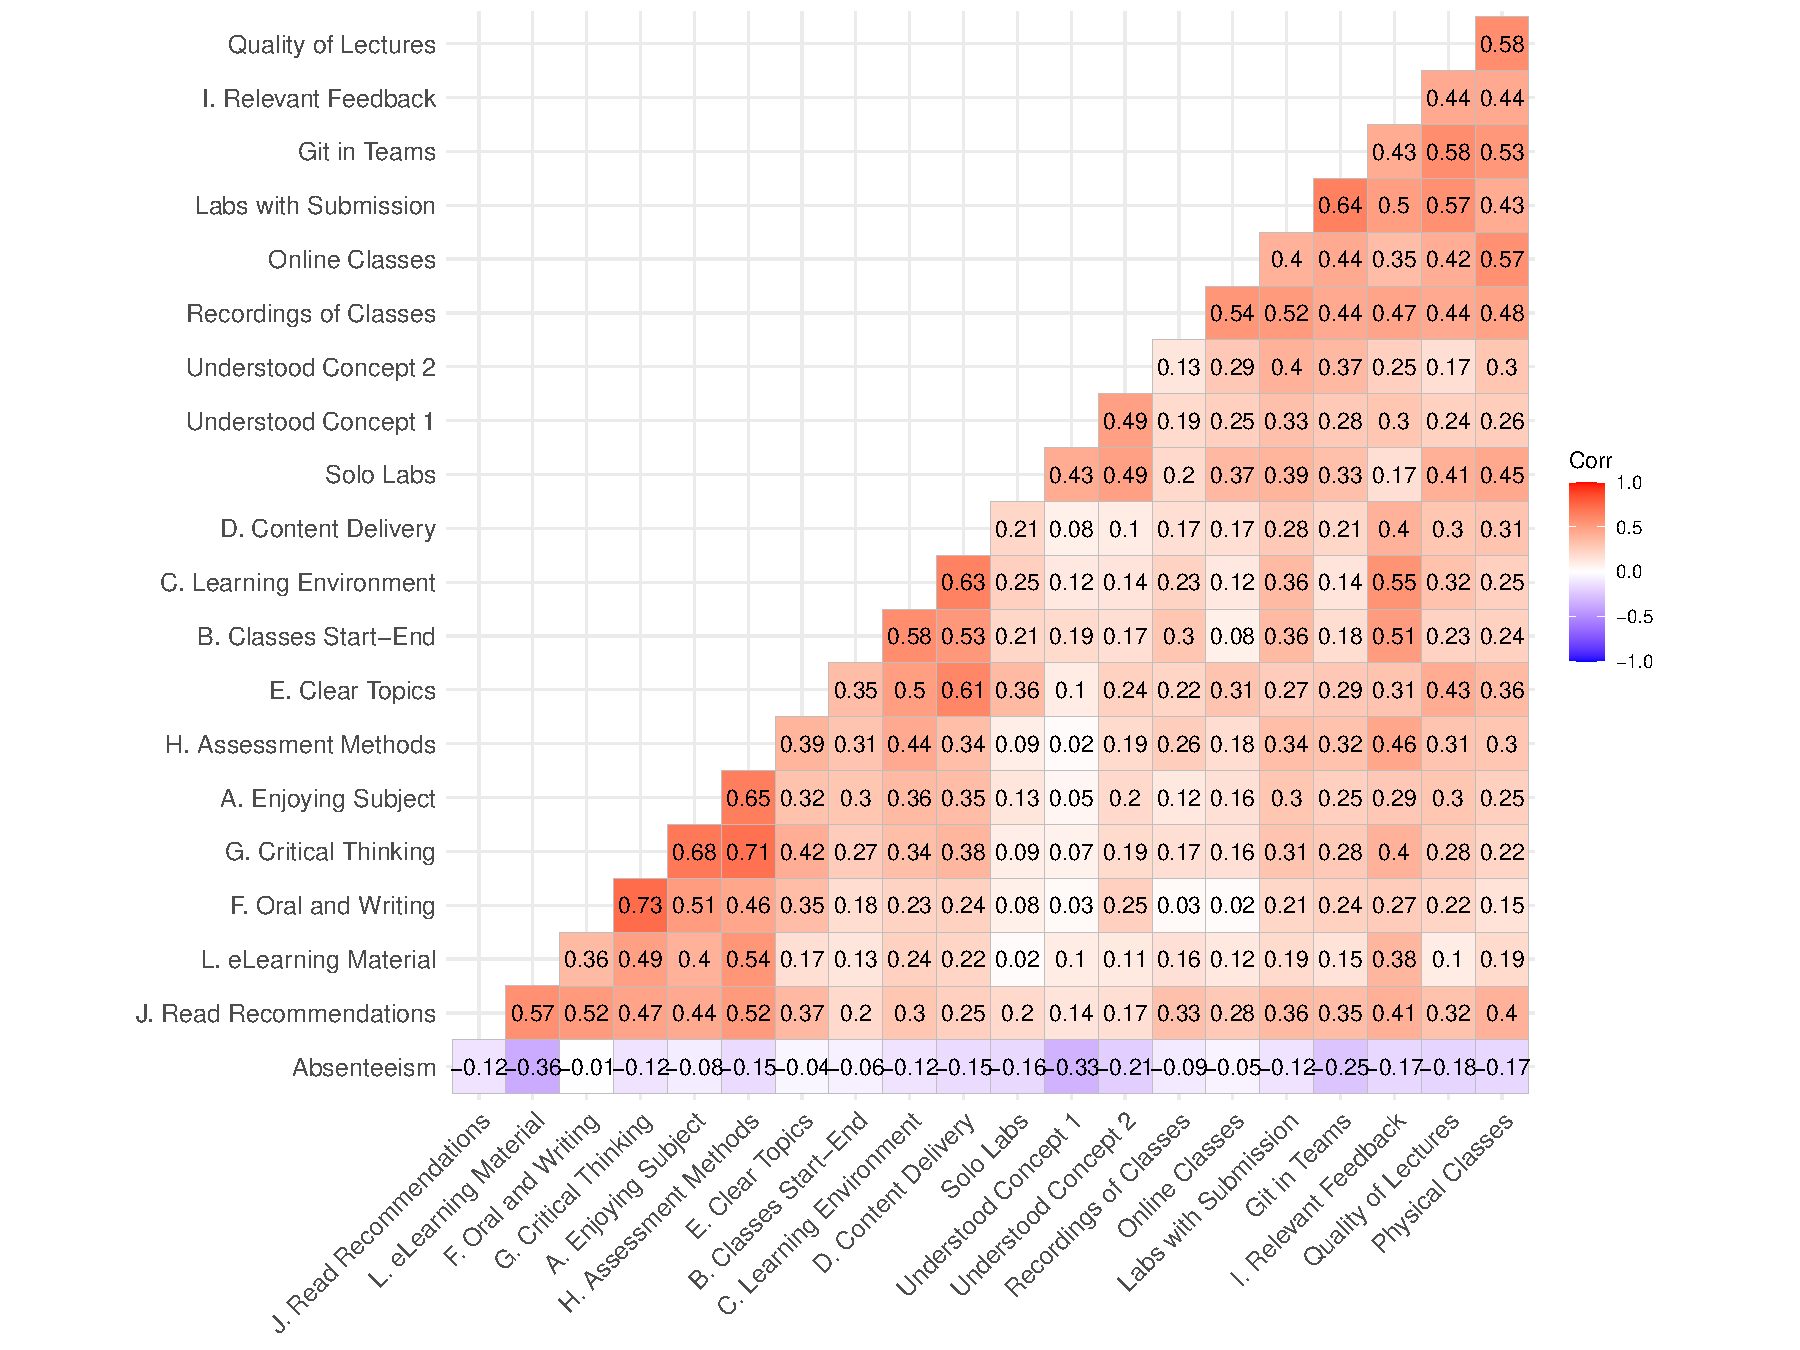
\includegraphics{AnalysisOfCourseEvaluation-Notebook_files/figure-latex/CorrelationMatrixWithFigures-1.pdf}

\subsection{Interesting Correlations}\label{interesting-correlations}

The following are hypothetical statements given that ``correlation does
not imply causation''.

\begin{itemize}
\item
  \textbf{.73 correlation} between ``I am developing my oral and writing
  skills'' and ``I am developing my reflective and critical reasoning
  skills'': \emph{Consider writing as formalized thinking.}
\item
  \textbf{.71 correlation} between ``The assessment methods are
  assisting me to learn'' and ``I am developing my reflective and
  critical reasoning skills'': \emph{The more effort students put into
  the assessment, the more they develop their reflective and critical
  reasoning skills.}
\item
  \textbf{.68 correlation} between ``I am enjoying the subject'' and ``I
  am developing my reflective and critical reasoning skills'': \emph{The
  more a student enjoys the subject, the more they consider their
  reflective and critical reasoning skills as developing.}
\item
  \textbf{.65 correlation} between ``The assessment methods are
  assisting me to learn'' and ``I am enjoying the subject'':
  \emph{Students who value the assessments enjoy the subject more.}
\item
  \textbf{.64 correlation} between ``Labs that require you to use Git to
  work in a team'' and ``Labs that require you to put in effort to make
  a submission related to the content of the lab'': \emph{The more
  students appreciate the use of Git for working in teams, the more they
  appreciate labs that require a submission to be made.}
\item
  \textbf{.61 correlation} between ``The subject content is delivered
  according to the course outline and meets my expectations'' and ``The
  topics are clear and logically developed'': \emph{The more the course
  outline is followed, the clearer and more logically developed the
  topics are.}
\item
  \textbf{-.33 correlation} between ``Concept 1 of 4 - Ensemble Methods
  for Predictive Analytics'' and ``Absenteeism'': \emph{Students who
  started the semester late (high absenteeism), had a harder time
  understanding concept 1 which was covered at the beginning of the
  semester.}
\item
  \textbf{-.36 correlation} between ``I use the e-learning material
  posted'' and ``absenteeism'': \emph{The higher the number of classes
  missed, the lower the student's engagement with content posted on
  e-learning}
\end{itemize}

Below are the two most extreme (positive and negative) correlations:

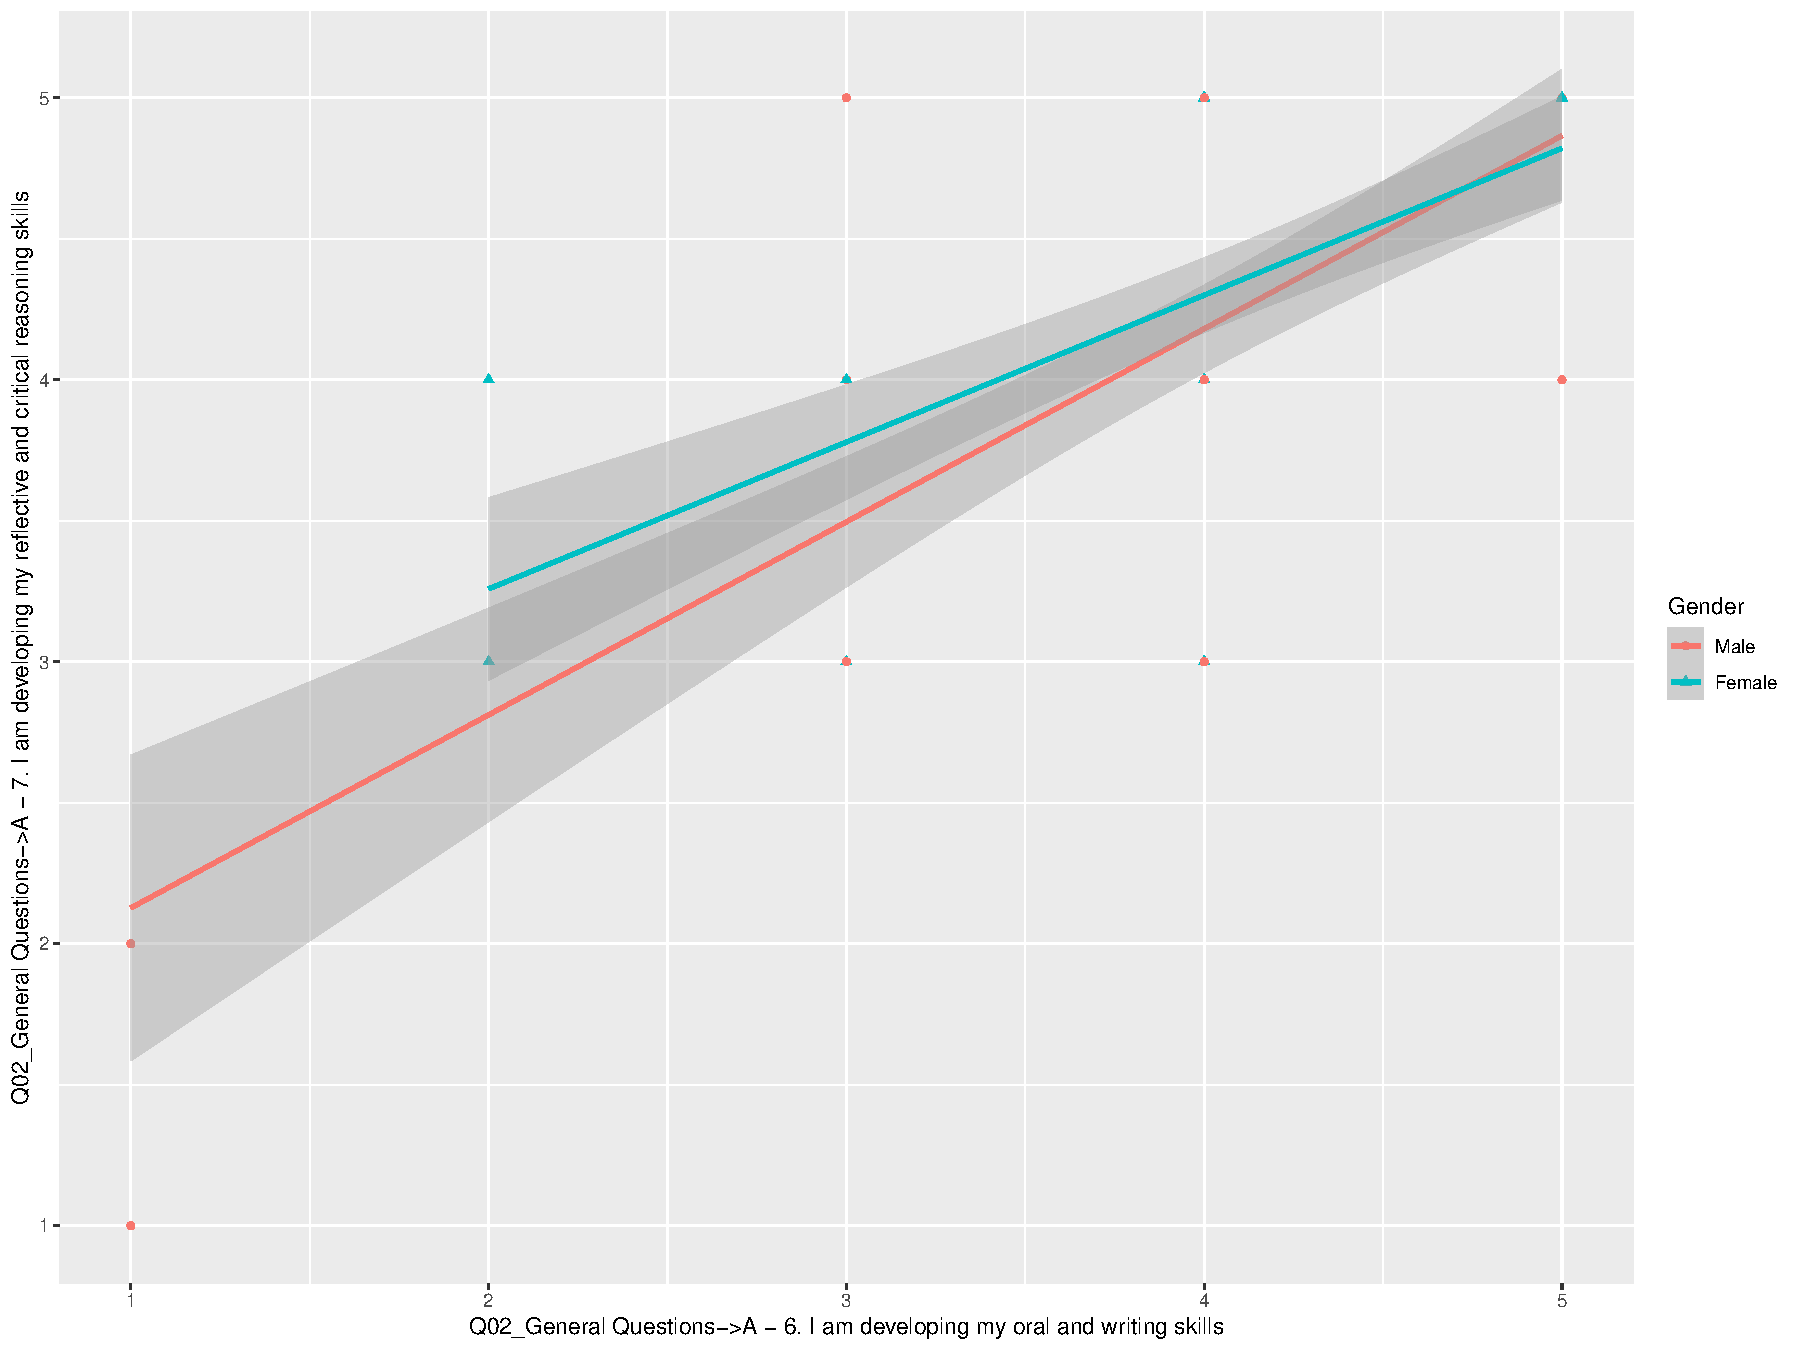
\includegraphics{AnalysisOfCourseEvaluation-Notebook_files/figure-latex/DrillDownCorr1-1.pdf}

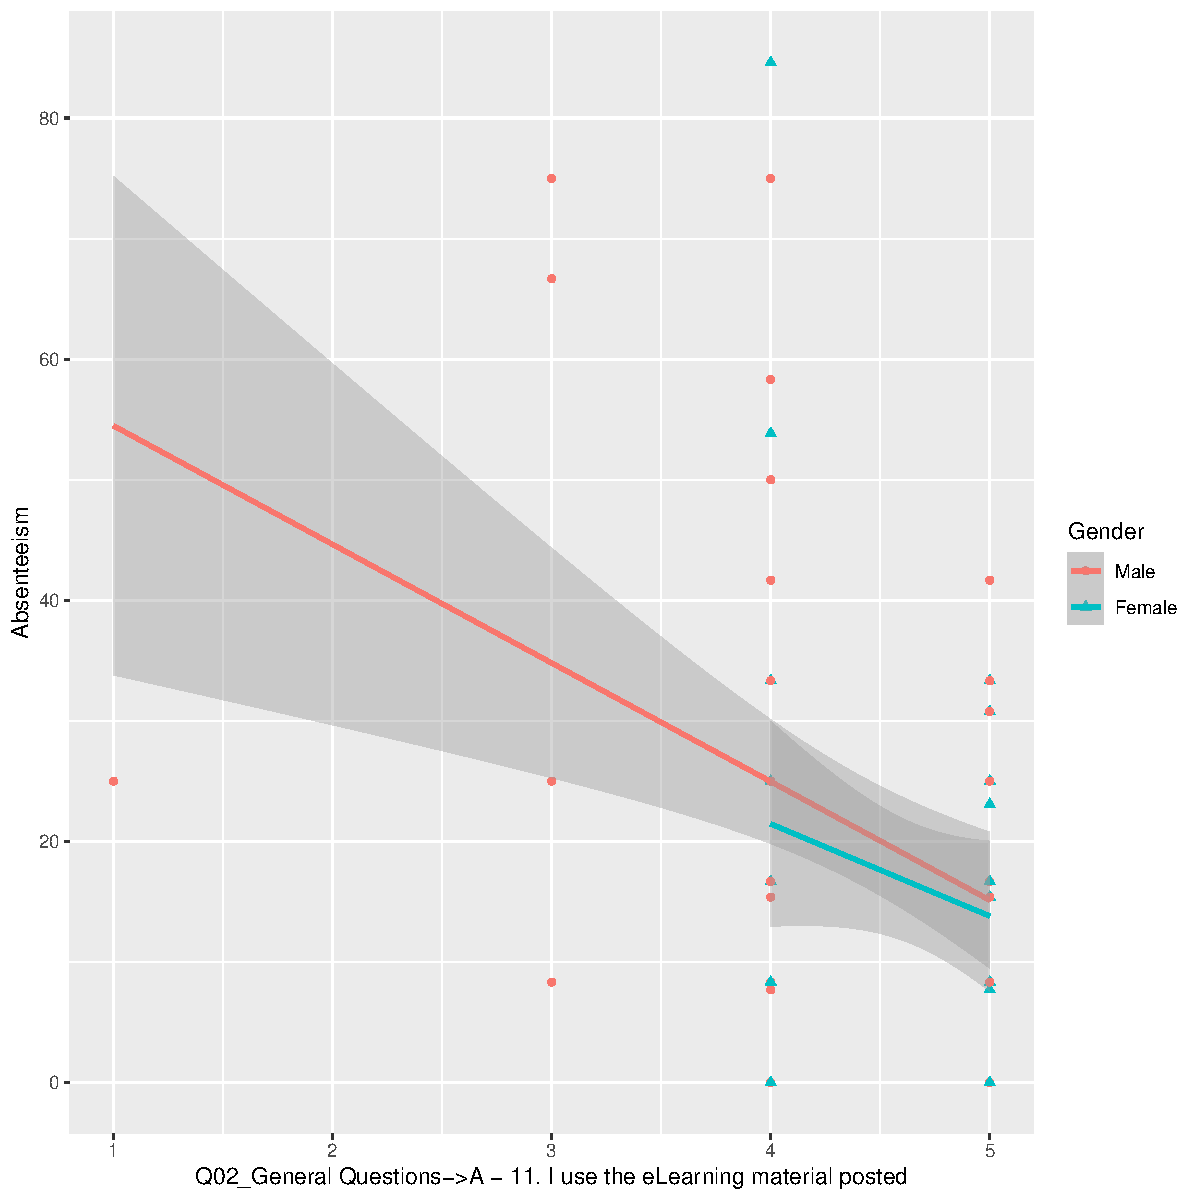
\includegraphics{AnalysisOfCourseEvaluation-Notebook_files/figure-latex/DrillDownCorr2-1.pdf}

\end{document}
